\section{Event displays}
\label{app:event-displays}
This appendix present a series of event displays from MC16e \powpyt{} samples for events that pass the analysis selection (a selection from the 20 first events in our test file).
Figure~\ref{fig:event-display-1} shows an event where one of the track jets falls on top of the leading muon. This hadronic activity appears to bias the reconstructed muon momentum high. 
Figure~\ref{fig:event-display-3} displays an event with many particles: more than 100 charged truth hadrons.
Figure~\ref{fig:event-display-4} shows an event for which a particle approximately 0.4 radians away from the jet core is included in the leading jet at reco level, but not at truth level, resulting in a shift of the jet axis.
Figure~\ref{fig:event-display-5} presents an event with several fake tracks. Likely due to a significant pileup interaction occuring ``close enough'' to the hard-scatter vertex.
Figure~\ref{fig:event-display-6} shows an event with many jets.


\begin{figure}[h!]
  \centering
  \includegraphics[page=6,width=0.48\textwidth]{figures/EventDisplays.pdf}
  \includegraphics[page=7,width=0.48\textwidth]{figures/EventDisplays.pdf} \\
  \includegraphics[page=9,width=0.48\textwidth]{figures/EventDisplays.pdf}
  \includegraphics[page=10,width=0.48\textwidth]{figures/EventDisplays.pdf}
  \caption{Event display for an event that passes all cuts (jet on top of muon).}
  \label{fig:event-display-1}
\end{figure}

\begin{figure}[h!]
  \centering
  \includegraphics[page=11,width=0.48\textwidth]{figures/EventDisplays.pdf}
  \includegraphics[page=12,width=0.48\textwidth]{figures/EventDisplays.pdf} \\
  \includegraphics[page=14,width=0.48\textwidth]{figures/EventDisplays.pdf}
  \includegraphics[page=15,width=0.48\textwidth]{figures/EventDisplays.pdf}
  \caption{Event display for an event that passes all cuts (quite event).}
  \label{fig:event-display-2}
\end{figure}

\begin{figure}[h!]
  \centering
  \includegraphics[page=21,width=0.48\textwidth]{figures/EventDisplays.pdf}
  \includegraphics[page=22,width=0.48\textwidth]{figures/EventDisplays.pdf} \\
  \includegraphics[page=24,width=0.48\textwidth]{figures/EventDisplays.pdf}
  \includegraphics[page=25,width=0.48\textwidth]{figures/EventDisplays.pdf}
  \caption{Event display for an event that passes all cuts (lots of particles).}
  \label{fig:event-display-3}
\end{figure}

\begin{figure}[h!]
  \centering
  \includegraphics[page=61,width=0.48\textwidth]{figures/EventDisplays.pdf}
  \includegraphics[page=62,width=0.48\textwidth]{figures/EventDisplays.pdf} \\
  \includegraphics[page=64,width=0.48\textwidth]{figures/EventDisplays.pdf}
  \includegraphics[page=65,width=0.48\textwidth]{figures/EventDisplays.pdf}
  \caption{Event display for an event that passes all cuts (skewed leading jet).}
  \label{fig:event-display-4}
\end{figure}

\begin{figure}[h!]
  \centering
  \includegraphics[page=81,width=0.48\textwidth]{figures/EventDisplays.pdf}
  \includegraphics[page=82,width=0.48\textwidth]{figures/EventDisplays.pdf} \\
  \includegraphics[page=84,width=0.48\textwidth]{figures/EventDisplays.pdf}
  \includegraphics[page=85,width=0.48\textwidth]{figures/EventDisplays.pdf}
  \caption{Event display for an event that passes all cuts (several fake tracks).}
  \label{fig:event-display-5}
\end{figure}

\begin{figure}[h!]
  \centering
  \includegraphics[page=96,width=0.48\textwidth]{figures/EventDisplays.pdf}
  \includegraphics[page=97,width=0.48\textwidth]{figures/EventDisplays.pdf} \\
  \includegraphics[page=99,width=0.48\textwidth]{figures/EventDisplays.pdf}
  \includegraphics[page=100,width=0.48\textwidth]{figures/EventDisplays.pdf}
  \caption{Event display for an event that passes all cuts (lots of jets).}
  \label{fig:event-display-6}
\end{figure}

